\documentclass[]{beamer}
 
\usepackage[utf8]{inputenc} 
\usepackage[T1]{fontenc}
\usepackage{lmodern}
\usepackage{graphicx}
\usepackage[french]{babel}
\usepackage{tikz}
\usepackage{listings}
 %\useoutertheme[subsection=false]{smoothbars}


\usetheme{Warsaw}
%\usetheme{Madrid}
%\usetheme{Frankfurt}
\setbeamertemplate{navigation symbols}{\insertframenumber/\,\inserttotalframenumber}

\begin{document}
 %\hspace*{1cm} \insertframenumber\,/\,\inserttotalframenumber
\title[Inférence de la structure d'une page web]{Inférence de la structure d'une page web en vue d'améliorer son accessibilité}
\subtitle[\ldots]{Encadré par : Marianne Huchard, Michel Meynard \& Yoann Bonnavero}
\author[PETITDEMANGE Franck]{PETITDEMANGE Franck}
\institute[LIRMM]{
\includegraphics[width=3cm]{img/Logo-lirmm.jpg}}
\date{27 juin 2014}
%\setbeamertemplate{footline}[page number]




\begin{frame}
\titlepage
\end{frame}

\section{Contexte du stage} 

\begin{frame}
\frametitle{Accessibilité du web}
\begin{columns}
	\begin{column}{4cm}
	\begin{definition}{Accessibilité}
	Capacité d'accéder aux informations contenues dans une page et d'interagir avec.
	\end{definition}
	\visible<2->{
	\begin{alertblock}{Problèmes d'accessibilité}
	\begin{itemize}
	\item Surcharge visuelle
	\item Police de caractère
	\item Contrastes de couleur
	\end{itemize}
	\end{alertblock}}
	\end{column}
	\begin{column}{4cm}
	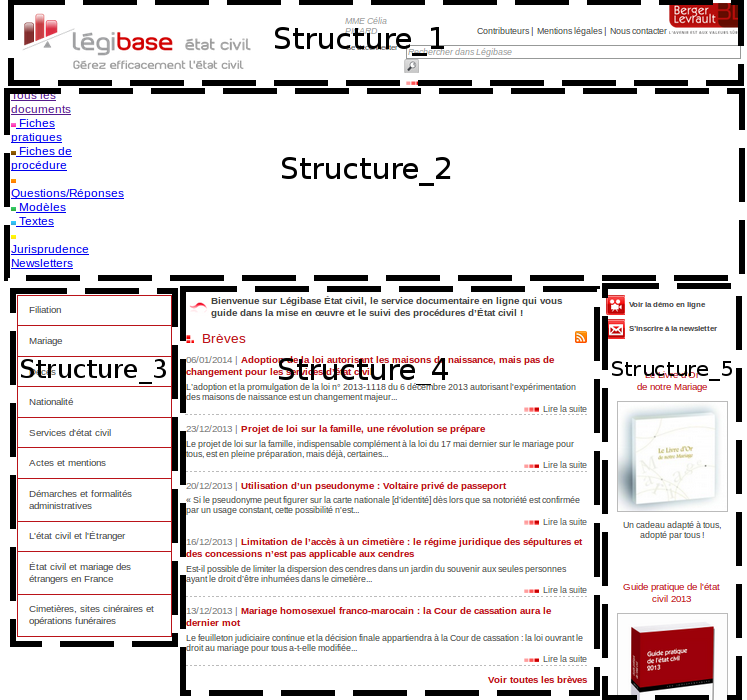
\includegraphics[scale=0.2]{img/segmentation_page_berger.png}
	\end{column}
\end{columns}
\end{frame}


\begin{frame}
	\frametitle{Approche générale}
\end{frame}

\begin{frame}
  \frametitle{Sommaire}
  \tableofcontents
\end{frame}

\section{Introduction} 
\begin{frame}
  \frametitle{Sommaire}
  \tableofcontents[currentsection, hideothersubsections]
\end{frame}

\begin{frame}
\end{frame}

\section{État de l'art}
\subsection{Étude des Langages de publication}
\begin{frame}
\frametitle{Description des fonctions}
\begin{columns}
	\begin{column}{4cm}
	\begin{block}{HTML 4}
	\end{block}
	\begin{block}{HTML 5}
	\end{block}
	\begin{block}{ARIA}
	\end{block}
	\end{column}
	\begin{column}{4cm}
	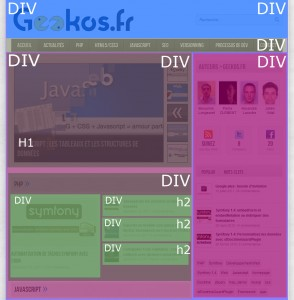
\includegraphics[scale=0.5]{img/architecture_HTML4.jpg}
	\end{column}
\end{columns}
\end{frame}
\begin{frame}
\frametitle{Description de la mise en forme}
\begin{columns}
	\begin{column}{4cm}
	\begin{block}{CSS}
	\end{block}
	\end{column}
	\begin{column}{4cm}
	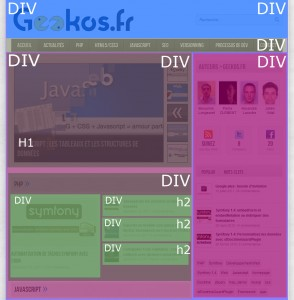
\includegraphics[scale=0.5]{img/architecture_HTML4.jpg}
	\end{column}
\end{columns}\end{frame}
\subsection{Étude de méthodes d'extraction de structure}
\begin{frame}
\frametitle{Mapping}
\end{frame}

\begin{frame}
\frametitle{Segmentation}
\framesubtitle{par pattern de présentation}
\end{frame}

\begin{frame}
\frametitle{Segmentation}
\framesubtitle{par densitométrie de textuelle }
\end{frame}

\begin{frame}
\frametitle{Segmentation}
\framesubtitle{par indice visuel}
\end{frame}

\begin{frame}
\frametitle{Synthèse}
\begin{block}{}
les inconvénients
\end{block}
\begin{block}{Notre approche}
\end{block}
\end{frame}

\section{Réalisation}
\begin{frame}
\end{frame}




 
\end{document}